\documentclass[sigconf, nonacm, review]{acmart}
\usepackage{graphicx}
\renewcommand\footnotetextcopyrightpermission[1]{} 
\settopmatter{printacmref=false}
\pagestyle{plain}
\begin{document}


\title{The title}
\subtitle{Accelerator-Centric Computing Ecosystems -- Programming Assignment Report }

%%
%% The "author" command and its associated commands are used to define
%% the authors and their affiliations.
%% Of note is the shared affiliation of the first two authors, and the
%% "authornote" and "authornotemark" commands
%% used to denote shared contribution to the research.


\author{Klemen Janez Poličar}
\email{k.j.policar@student.vu.nl}
\affiliation{%
  \institution{Computer Science, VU Amsterdam}
  \country{}
}

\author{Author 2}
\email{author2@mail.com}
\affiliation{%
  \institution{Computer Science, VU Amsterdam}
  \country{}
}
\author{Author 3}
\email{author3@mail.com}
\affiliation{%
  \institution{Computer Science, VU Amsterdam}
  \country{}
}


%%
%% The abstract is a short summary of the work to be presented in the
%% article.
\begin{abstract}
  [Optional]  a high-level description of your solution, analysis overview, and main results
\end{abstract}




%%
%% This command processes the author and affiliation and title
%% information and builds the first part of the formatted document.
\maketitle

\section{Introduction}
A brief overview of the problem, motivation for GPU acceleration, and the structure of the remainder of the article. Use one short paragraph for each.\\

\noindent
\textit{Note: you are allowed to deviate from this template as long as the same information is included and it is clear where it is discussed.}

\section{Parallelization}
\textbf{Parallelizable sections and identification.}
We analyzed loop dependencies in the reference code and found that Step 2 (spillage computation) and Step 3 (water update) are grid-wide passes where each iteration operates on one cell with the same arithmetic pattern. These phases dominate runtime and are therefore mapped to CUDA kernels. Step 1 (cloud movement and rainfall) was initially kept on the CPU to keep the first GPU version simple and easy to validate.

\textbf{Workload distribution (geometry).}
We use a 2D CUDA launch where each thread is responsible for one matrix cell $(row,col)$. Blocks are configured as $16\times16$, and the grid dimensions are computed from the terrain size. This mapping follows the natural 2D structure of the terrain and provides regular parallel work across the full domain.

\textbf{Applied optimizations.}
As a first optimization step, we move the expensive per-cell phases to the GPU while preserving the original algorithm. Device buffers for ground and auxiliary arrays are allocated once and reused across iterations. We also use low-overhead reductions via atomics for global metrics (maximum spillage per iteration and boundary water loss), and unroll the fixed 4-neighbor loop to reduce instruction overhead.

\section{Implementation details}
If not already included in the previous section.

\section{Evaluation}

\subsection{Experimental setup}
All measurements were taken on DAS-5 nodes equipped with NVIDIA GeForce GTX Titan X GPUs, using CUDA 12.6. Timing uses the wall-clock \texttt{get\_time()} wrapper around the simulation loop only (excluding allocation and initialization).

\subsection{Step 1: Initial GPU port}
After moving the spillage computation and water update phases to two CUDA kernels (keeping cloud movement and rainfall on the CPU), we benchmarked all reference inputs against the sequential version.

\begin{center}
\begin{tabular}{lrrr}
\hline
\textbf{Input} & \textbf{Seq (s)} & \textbf{CUDA (s)} & \textbf{Speedup} \\
\hline
\texttt{debug}             &   0.085 &   0.029 &  2.9$\times$ \\
\texttt{small\_mountains}  &   0.045 &   0.018 &  2.5$\times$ \\
\texttt{custom\_clouds}    &   0.342 &   0.166 &  2.1$\times$ \\
\texttt{medium\_lower\_dam}&   0.976 &   0.169 &  5.8$\times$ \\
\texttt{medium\_higher\_dam}&  0.995 &   0.139 &  7.1$\times$ \\
\texttt{large\_mountains}  & 181.359 &  15.196 & 11.9$\times$ \\
\hline
\end{tabular}
\end{center}

Speedups range from $\sim$2$\times$ on small inputs to $\sim$12$\times$ on the largest, but remain below the 20$\times$ target. To understand the bottleneck, we profiled with \texttt{nvprof}.

\subsection{Profiling with nvprof}
We ran \texttt{nvprof} on every input. The table below shows the fraction of GPU time spent on host$\leftrightarrow$device memory transfers versus actual kernel compute:

\begin{center}
\begin{tabular}{lrrr}
\hline
\textbf{Input} & \textbf{Grid} & \textbf{Memcpy \%} & \textbf{Kernel \%} \\
\hline
\texttt{debug}              & $90\times90$     & 41\% & 54\% \\
\texttt{small\_mountains}   & $100\times100$   & 45\% & 50\% \\
\texttt{custom\_clouds}     & $120\times120$   & 47\% & 49\% \\
\texttt{medium\_lower\_dam} & $400\times300$   & 60\% & 39\% \\
\texttt{medium\_higher\_dam}& $256\times256$   & 62\% & 37\% \\
\texttt{large\_mountains}   & $3072\times2048$ & 74\% & 26\% \\
\hline
\end{tabular}
\end{center}

A clear trend emerges: as grid size grows, memory transfers dominate increasingly --- reaching \textbf{74\% of GPU time} on the largest input. This happens because the initial implementation copies the entire \texttt{water\_level} array to the device and back \emph{every iteration}: once so the GPU kernels can read the CPU-updated rainfall, and once to bring results back for the next CPU rainfall pass. On \texttt{large\_mountains} with 800 iterations, this produces over 2400 \texttt{cudaMemcpy} calls totalling 6.5\,s of transfer time.

Figure~\ref{fig:step1} visualizes this breakdown: each bar shows total execution time split into kernel compute (blue), memory transfers (orange), and remaining CPU/overhead (grey).

\begin{figure}[h]
\centering
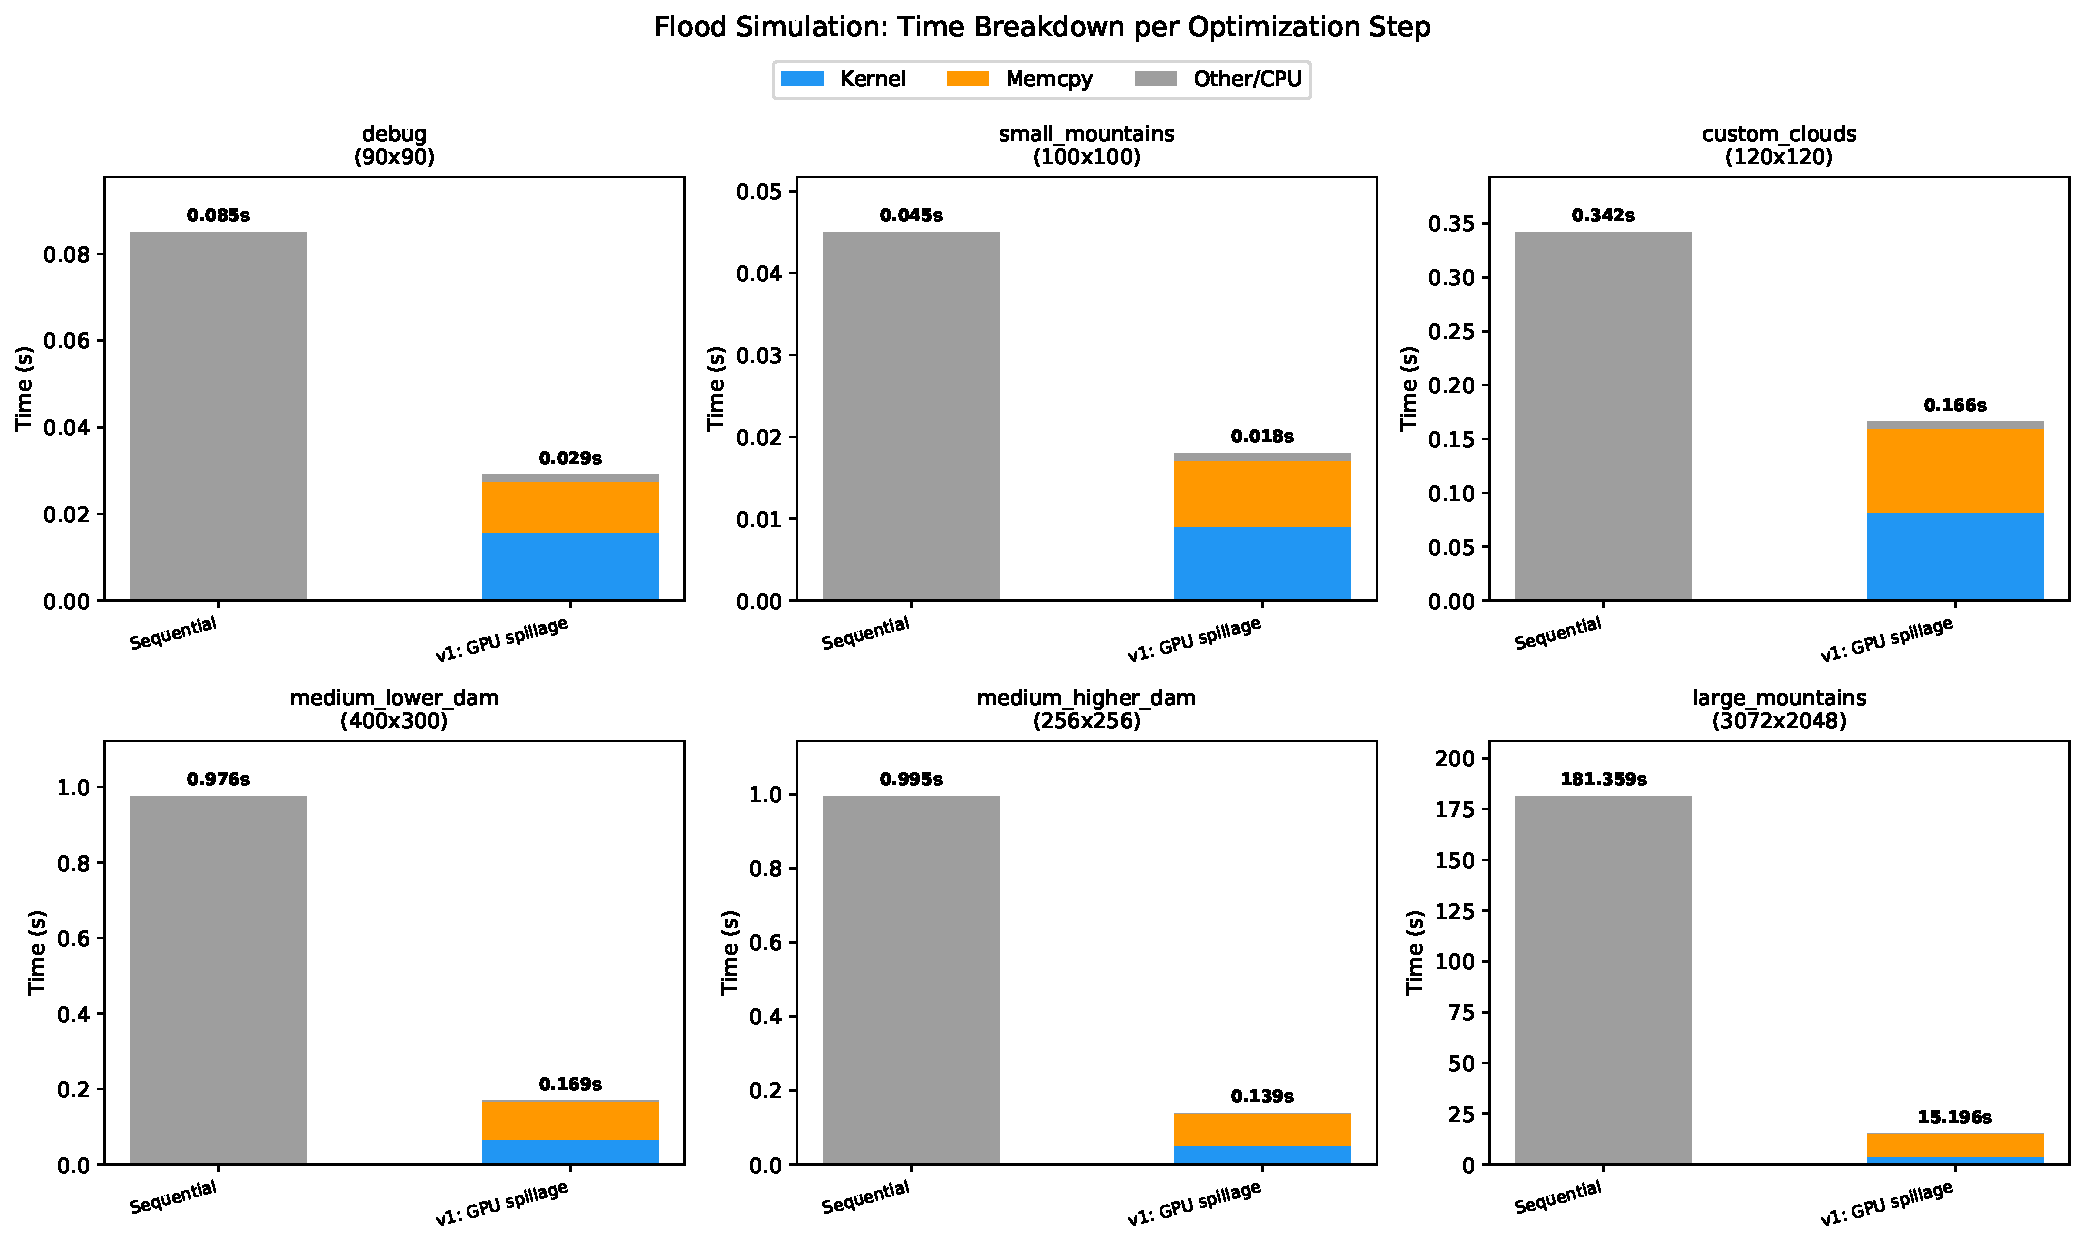
\includegraphics[width=\linewidth]{perf_breakdown.pdf}
\caption{Time breakdown after Step~1 (GPU spillage). Sequential time is entirely CPU; the CUDA version splits into kernel, memcpy, and overhead. Memory transfers dominate on larger inputs.}
\label{fig:step1}
\end{figure}

This profiling result points to a clear next optimization target: \textbf{move the rainfall computation to the GPU} so that \texttt{water\_level} can remain on the device across iterations, eliminating the per-iteration round-trip transfers.

\section{Discussion and Conclusion}

Describe the challenges, limitations, and possible optimizations to your solution. We expect you to provide a summary of your findings and (Optional but encouraged) lessons learned and time sheets (report the time it took to conduct each major part of the assignment.


%% The next two lines define the bibliography style to be used, and
%% the bibliography file.
\bibliographystyle{ACM-Reference-Format}
\bibliography{sample-base}
\end{document}